\documentclass[paper=letter, fontsize=12pt]{scrartcl} % Letter paper and 12pt font size
\usepackage{amssymb, graphicx, amsmath, amsfonts, enumerate, booktabs, multirow, fancyvrb, hyperref, xcolor}
\usepackage[brazilian]{babel}
\usepackage[utf8]{inputenc}
\usepackage[T1]{fontenc}
\newcommand{\ep}{\vspace*{.05in}}
\newcommand{\eg}{\vspace*{.7cm}}

\usepackage{fourier} % Use the Adobe Utopia font for the document - comment this line to return to the LaTeX default

\usepackage{float}
\usepackage{lipsum} % Used for inserting dummy 'Lorem ipsum' text into the template

\usepackage{sectsty} % Allows customizing section commands
\allsectionsfont{\centering \normalfont\scshape} % Make all sections centered, the default font and small caps

\usepackage[left=1in, top=1in, right=1in, bottom=1in, headsep=50pt]{geometry}

\usepackage{lastpage}

\usepackage{fancyhdr}
\pagestyle{fancyplain}
\fancyhead{} % Clear all header fields
\fancyfoot{}
%\fancyfoot[C]{\thepage} % Page numbering for center footer
\fancyfoot[R]{} % Page numbering for right footer
\fancyhead[L]{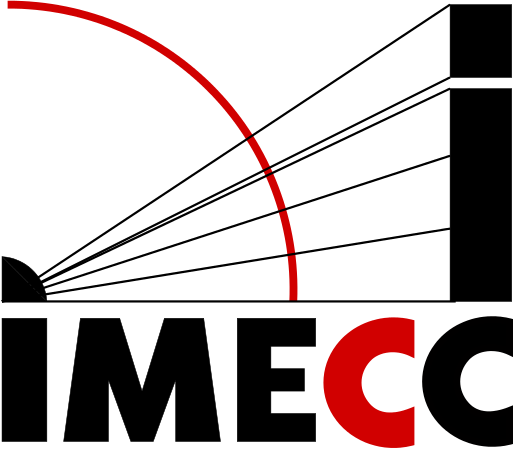
\includegraphics[height=.6in]{logo-imecc}
\begin{small}\hspace{2.5cm} Departamento de Estat\'istica - IMECC - UNICAMP - Página \thepage /\pageref{LastPage} \end{small}
\hfill{
\includegraphics[height=.6in]{unicamp}}
\horrule{0.5pt}
}
\renewcommand{\headrulewidth}{0pt} % Remove header underlines
\renewcommand{\footrulewidth}{0pt} % Remove footer underlines

\setlength\parindent{0pt} % Removes all indentation from paragraphs - comment this line for an assignment with lots of text

\newcommand{\horrule}[1]{\rule{\linewidth}{#1}} % Create horizontal rule command with 1 argument of height

\title{\normalfont \LARGE ME414C - Estatística para Experimentalistas}
\subtitle{1º Semestre de 2022}
\author{}
\date{}

\begin{document}

\maketitle

\vspace{-1.5cm}

\noindent
\begin{tabular}{rl}
\textbf{Professor:} & 	 Benilton Carvalho \\
\textbf{PED:} 	    & Robinson Ortega Meza \\
\\
\textbf{Aulas:} & Segundas 21h-23h - CB05\\
                & Quintas 19h-21h - CB02 \\
\textbf{Atendimento:} & Será divulgado no Moodle\\

 % Link do Google Meet: \href{https://meet.google.com/yor-ahij-xem}{{\color{blue}https://meet.google.com/yor-ahij-xem}}.\\ O mesmo link será utilizado em caso de necessidade de aulas remotas.\\


\end{tabular}

\section{Informações Gerais e Normas}

\begin{itemize}

\item A leitura da ementa em sua integralidade é fortemente recomendada, não cabendo aos alunos desculpas por ignorância quanto ao seu conteúdo.

\item Comunicação por email: em casos extremamente particulares e individuais, APENAS pelo email institucional, especificando [ME414C], no assunto da mensagem e APENAS remetentes de emails xxx.unicamp.br. Qualquer outra mensagem sem essas especificações será ignorada. Perguntas sobre o conteúdo, exercícios, etc..., devem ser TODAS encaminhadas ao Fórum que está no Moodle.

\item Os alunos regularmente matriculados estarão inscritos automaticamente no Moodle da disciplina:

\hspace{3cm} \href{https://moodle.ggte.unicamp.br/course/view.php?id=13073}{{\color{blue} ME414C}}

% \hspace{3cm} \href{https://moodle.ggte.unicamp.br/course/view.php?id=12763}{{\color{blue} ME111B}}

% {\color{red} Os alunos da turma ME111B serão transferidos para o Moodle da disciplina ME111A.}

O aluno deverá logar com o mesmo usuário e senha usado para acessar os serviços da DAC. O login usado para acessar o Moodle é intransferível (\href{http://www.pg.unicamp.br/mostra_norma.php?id_norma=3256}{{\color{blue} GR-052/2012 , Capítulo VI, artigo 59}}).

\item Informações relevantes referentes às atividades de avaliação serão disponibilizadas na página do Moodle citada acima.

\item As atividades de avaliação no Moodle têm data de fechamento. O aluno deverá submetê-las antes da data especificada para receber a nota.

\item Caso a aula seja transmitida de maneira remota, o aluno deve acessar o \textit{Google Meet} nos horários indicados usando a conta de e-mail institucional (email Unicamp). O link será divulgado na ocasião.

\item O professor da disciplina não é direta ou indiretamente responsável pela administração dos sistemas computacionais da universidade. O aluno deverá dirigir-se aos responsáveis em caso de qualquer problema com os sistemas computacionais e serviços relacionados.

\item O código de honra deve ser preservado. O aluno deverá proceder de forma respeitosa e honesta durante as aulas, bem como na resolução de qualquer outra atividade que seja parte da avaliação do curso.

\item Casos não contemplados neste documento serão devidamente avaliados.

\end{itemize}

\section{Protocolos COVID}

\begin{itemize}

\item Todos os alunos deverão usar máscara (idealmente PFF2 ou N95) durante toda a sua estadia na sala de aula. Caso o aluno necessite beber água, o aluno deverá se retirar, retornando apenas após a máscara estar devidamente colocada.

\item Caso o aluno esteja com sintomas de COVID, ou com COVID confirmada (com ou sem sintomas), ou teve contato com casos de COVID, conferir os \href{https://www.ime.unicamp.br/retomada/pros.html}{PRO's} (Protocolos Rápidos de Orientação). \textbf{Comunicar imediatamente ao professor, via email}. O aluno será instruído a realizar as atividades em domicílio, conforme sua condição de saúde, portanto é importante comunicar imediatamente.

\item Se houver mais de um caso confirmado de COVID na turma, as aulas migrarão para o formato remoto.

\item Caso o professor esteja com sintomas de COVID, ou com COVID confirmada (com ou sem sintomas) ou teve contato com casos de COVID, as aulas migrarão para o formato remoto.

\end{itemize}

\section{Freqüência}

Esta é uma disciplina com requerimento freqüência mínima de 75\% (\href{https://www.dac.unicamp.br/portal/graduacao/regimento-geral}{Art. 13 - VII - Regimento Geral de Graduação da UNICAMP}). Os abonos de falta ocorrerão de acordo com o descrito na \href{https://www.dac.unicamp.br/portal/graduacao/regimento-geral}{Seção X, Art. 72 do Regimento Geral de Graduação da UNICAMP}.

\section{Critérios de Avaliação}

A avaliação se dará através da realização das Provas 1 e 2, respectivamente, P1 e P2. No caso de ausência em uma das provas de acordo com os critérios de abono de faltas supracitados, o aluno poderá realizar o Exame para substituir a avaliação em que precisou faltar (\href{https://www.dac.unicamp.br/portal/graduacao/regimento-geral}{Art. 57, §4º - Regimento Geral da Graduação da UNICAMP}).

\vspace{10pt}

A Média Geral (MG) será dada pela seguinte fórmula:
\[MG = 0.35 P1 + 0.65 P2\]

\newpage

\textbf{Aprovação}

Pelo \href{https://www.dac.unicamp.br/portal/graduacao/regimento-geral}{{\color{blue} Regimento Geral de Graduação, Seção I, Artigo 57}}, estabelecemos os seguintes critérios para aprovação e exame.

\begin{itemize}
\item Se MG $\geq$ 6 \textbf{e} freqüência mínima de 75\%, o aluno está aprovado e MF = MG.

\item Se 2.5 $\leq$ MG < 6 \textbf{e} freqüência mínima de 75\%, o aluno deverá fazer o Exame (E).

\item Se MG < 2.5 \textbf{ou} freqüência mínima de 75\%, o aluno está reprovado e MF = MG.

\item Para o aluno que ficar de exame, a Média Final (MF) será:
$$MF = \min\left(6.0, \frac{MG + Exame}{2}\right)$$

Nesse caso, se MF $\geq$ 6, o aluno está aprovado. Caso contrário, está reprovado.


%\item Caso esteja aprovado, receberá conceito ``S''. Caso esteja reprovado, receberá conceito ``I''.
\end{itemize}

\section{Datas Importantes}

\begin{tabular}{ll}
09/Maio/2022  & P1 \\
14/Julho/2022 & P2 \\
25/Julho/2022 & Exame Final
\end{tabular}

\section{Outras Informações}

Outras informações estarão disponíveis por meio dos seguintes recursos:

\begin{itemize}
\item \href{https://moodle.ggte.unicamp.br/course/view.php?id=13073}{{\color{blue} ME414C - Moodle}}
\item \href{https://me414-unicamp.github.io}{{\color{blue} ME414 - Site}}
\end{itemize}

\section{Bibliografia}
\begin{enumerate}
\item Ross, S. M. (2010). \href{http://www.sciencedirect.com/science/book/9780123743886}{Introductory Statistics}.
\item Diez, D. M.; Barr, C. D.; Çetinkaya-Rundel, M. (2015). \href{https://leanpub.com/openintro-statistics}{OpenIntro Statistics}.
\item Magalhães, M.N. e de Lima, A.C.P. (2001) Noções de Probabilidade e Estatística IME-USP.
\item Devore, J. L. (2018). \href{http://acervus.unicamp.br/index.asp?codigo_sophia=1138563}{Probabilidade e estatística para engenharia e ciências}
\end{enumerate}


Para acessar alguns dos livros digitais remotamente, você precisará do VPN. Veja instruções de instalação \href{http://www.ccuec.unicamp.br/ccuec/acesso_remoto_vpn}{{\color{blue} aqui}}.


\end{document}
